% =============================================================================
\chapter{Method and Implementation}
\label{ch:method}
% =============================================================================
% PURPOSE: describes HOW every quantity of Chapter 3 is computed, so that the
% results of Chapter 5 can be reproduced and judged. It separates the
% measuring instrument (this chapter) from the measurements (Chapter 5). The
% last section sketches the singularity-aware extraction method required by
% the assignment; it is marked as work in progress.

This chapter describes the software written for the thesis and the numerical
methods behind each measurement. The guiding principle is that a measurement
of an extracted mesh should not depend on the same mesh for its reference:
wherever possible, distances, singular points and invariants are computed
from the polynomial itself, and the mesh is used only as a starting point.

% -----------------------------------------------------------------------------
\section{Overview}
\label{sec:method-overview}
% PURPOSE: a map of the software, so that later sections can refer to its parts.

The software consists of three layers (Figure~\ref{fig:architecture}): a
header-only C++17 library for parsing, evaluating and polygonizing implicit
functions; an analysis layer that implements the measurements of this
chapter; and an interactive viewer used for exploration and for the figures.
The experiments of Chapter~\ref{ch:experiments} are produced by a command-line
program, \texttt{isosurface\_thesis\_experiments}, which runs the same
analysis as the viewer without a graphical interface and writes all results
to CSV files.

\begin{figure}[!h]
\centering
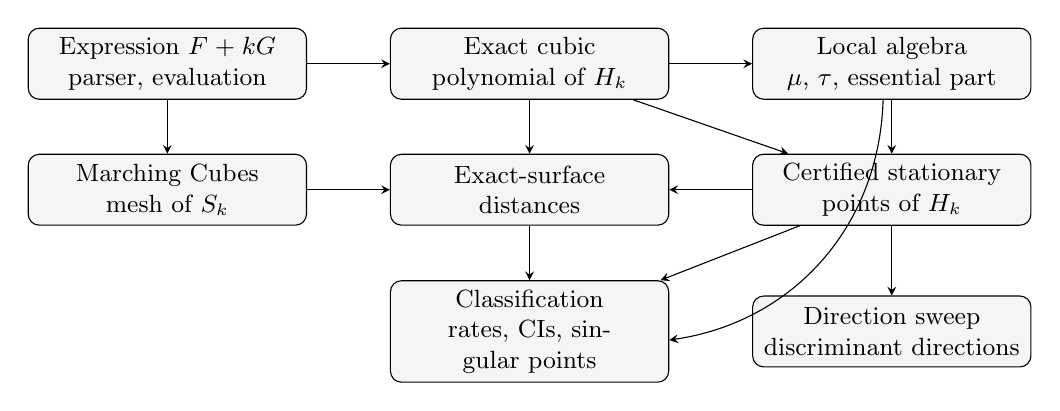
\begin{tikzpicture}[font=\small, box/.style={draw, rounded corners, align=center, minimum height=0.9cm, text width=3.3cm, fill=gray!8}, >=stealth]
    \node[box] (expr) at (0,0) {Expression $F+kG$\\parser, evaluation};
    \node[box] (mc) at (0,-1.6) {Marching Cubes\\mesh of $S_k$};
    \node[box] (poly) at (4.6,0) {Exact cubic\\polynomial of $H_k$};
    \node[box] (alg) at (9.2,0) {Local algebra\\ $\mu$, $\tau$, essential part};
    \node[box] (stat) at (9.2,-1.6) {Certified stationary\\points of $H_k$};
    \node[box] (exact) at (4.6,-1.6) {Exact-surface\\distances};
    \node[box] (cls) at (4.6,-3.4) {Classification\\rates, CIs, singular points};
    \node[box] (sweep) at (9.2,-3.4) {Direction sweep\\discriminant directions};
    \draw[->] (expr) -- (mc);
    \draw[->] (expr) -- (poly);
    \draw[->] (poly) -- (alg);
    \draw[->] (poly) -- (stat);
    \draw[->] (alg) -- (stat);
    \draw[->] (mc) -- (exact);
    \draw[->] (poly) -- (exact);
    \draw[->] (stat) -- (exact);
    \draw[->] (exact) -- (cls);
    \draw[->] (stat) -- (cls);
    \draw[->] (alg) to[bend left=40] (cls);
    \draw[->] (stat) -- (sweep);
\end{tikzpicture}
\caption[Analysis pipeline]{The analysis pipeline. The mesh enters only the
distance computation, and there only as a source of starting points.}
\label{fig:architecture}
\end{figure}

For every perturbation $G$ and every sampled $k$, the analysis extracts the
mesh once and then computes, in parallel over $k$:
the certified stationary points of $H_k$ (Section~\ref{sec:method-stationary}),
the local Hausdorff distance between the exact surfaces $S_k$ and $S_0$
(Section~\ref{sec:method-exact}), and the geometric accuracy of the mesh
(Section~\ref{sec:method-accuracy}). The local algebra of $F$
(Section~\ref{sec:method-algebra}) is computed once per surface.

% -----------------------------------------------------------------------------
\section{Isosurface Extraction}
\label{sec:method-extraction}
% PURPOSE: the extraction method whose behaviour near singularities is
% studied; the details listed here (node layout, tie-break) influence the
% results and must be documented.

The surfaces are extracted with the Marching Cubes algorithm of
Section~\ref{sec:marching-cubes} \cite{lorensen1998marching} on the uniform grid with nodes
$-L+2Li/N$, $i=0,\dots,N$, in each coordinate, where $[-L,L]^3$ is the domain
and $N$ the number of cells per axis; the grid spacing is $h=2L/N$. For even
$N$ the origin is a grid node. Each cut edge is interpolated once
(Definition~\ref{def:edge-interp}), so neighbouring cells share their vertices
exactly.

\paragraph{Grid nodes on the surface.}
A node at which $F$ vanishes would make several edge intersections collapse
onto the node and produce degenerate triangles. The real lines of the cones
pass through many grid nodes (for example the line $x=-y$, $z=0$ of $F_+$). A
node counts as \emph{on the surface} if $F=0$ there, or if $|F|$ is below
$10^{-10}$ times the largest value of $|F|$ at its six neighbours, which
catches rounding noise. If such a node has neighbours of opposite signs, its
value is replaced by $5\%$ of the smallest nonzero neighbour value, a
deterministic tie-break towards the positive side. The analytic field is kept
for all later computations.

\paragraph{Normals.}
Vertex normals and gradient magnitudes are evaluated exactly at the vertices
by forward-mode automatic differentiation \cite{griewank2008evaluating}: the
expression is evaluated with dual numbers $a+b_x\varepsilon_x+b_y\varepsilon_y+b_z\varepsilon_z$,
which carry the gradient along with the value.

% -----------------------------------------------------------------------------
\section{Experimental Parameters}
\label{sec:method-parameters}
% PURPOSE: the choices that every number of Chapter 5 depends on, in one place.

\paragraph{Local box.} All local quantities are measured in the box
$Q_a=[-a,a]^3$ around the singular point with $a=0.18$, inside the domain
$[-0.4,0.4]^3$.

\paragraph{Resolutions.} The grids have $N=32$, $64$ and $128$ cells per axis,
with spacings $h=0.025$, $0.0125$ and $0.00625$. Doubling the resolution
halves $h$, which makes the dependence on $h$ directly visible.

\paragraph{Parameter values.} The rate of convergence is the slope of
$\log d_a(k)$ against $\log|k|$, so the samples are spaced uniformly in
$\log|k|$: nine values of $|k|$ between $10^{-4}$ and $10^{-2}$ on each side
of zero,
\begin{equation}
\label{eq:k-samples}
|k|=10^{-2-2j/8},\qquad j=0,\dots,8 .
\end{equation}
Uniformly spaced values in $k$ would put most samples at the large end of the
range and only one or two in the decade closest to zero.

% -----------------------------------------------------------------------------
\section{Distances on the Exact Surfaces}
\label{sec:method-exact}
% PURPOSE: the main improvement over a mesh-to-mesh comparison. A distance
% between two meshes mixes the change of the surface with the extraction
% errors of both meshes; this section measures the change of the surface
% itself, which is the quantity the theory predicts.

Comparing two extracted meshes measures the change of the surface plus the
extraction errors of both meshes, and the errors are of the order of the grid
spacing $h$. When the deformation is smaller than $h$, the comparison measures
mainly the errors. The local Hausdorff distance $d_a(S_k,S_0)$ is therefore
computed between the exact surfaces, with the meshes serving only to find
starting points. This requires two operations: moving a point onto a surface,
and computing the distance from a point to a surface.

\paragraph{Moving a point onto the surface.}
A point $p$ near $S=\{H=0\}$ is moved onto $S$ by Newton's method along the
gradient,
\begin{equation}
\label{eq:projection}
p\leftarrow p-\frac{H(p)}{\|\nabla H(p)\|^2}\,\nabla H(p),
\end{equation}
with each step limited to one grid spacing. The iteration stops when the step
is at rounding level; it is accepted if $|H(p)|$ is then below $10^{-10}$ times
the sum of the absolute values of the terms of $H$ at $p$. Near a singular
point the gradient vanishes and the iteration can fail; such points are
counted and reported.

\paragraph{Distance from a point to the surface.}
The closest point $p$ of $S$ to a point $b$ satisfies the Lagrange conditions
of minimizing $\|p-b\|^2$ subject to $H(p)=0$ \cite{nocedal2006numerical},
\begin{equation}
\label{eq:lagrange}
p-b+\lambda\nabla H(p)=0,\qquad H(p)=0,
\end{equation}
four equations in the unknowns $p$ and $\lambda$. They are solved by Newton's
method, with the Jacobian
$\left(\begin{smallmatrix}I+\lambda\operatorname{Hess}H & \nabla H\\ \nabla H^{\top} & 0\end{smallmatrix}\right)$,
started at a point of $S$. Newton's method finds a nearby solution of
\eqref{eq:lagrange}, which is the closest point if the start is close enough,
but may be another critical point of the distance otherwise. Two starts are
used: the closest point of the mesh of $S$ (computed exactly with a bounding
volume hierarchy and the closest-point-on-triangle routine of
\cite{ericson2004realtime}), moved onto $S$; and the nearest exact sample of
$S$ found so far. The result is the smallest of the distances to these two
points, to the two Newton solutions, and to the singular points of $S$, which
are known from Section~\ref{sec:method-stationary} and where
\eqref{eq:lagrange} degenerates. Every candidate is an exact point of $S$, so
the result is never smaller than the true distance; it equals it whenever one
of the starts lies in the basin of the closest point.

\paragraph{Samples and graded refinement towards the singular point.}
The supremum in Definition~\ref{def:local-hausdorff} is taken over samples:
the vertices and triangle centroids of the mesh inside the box, moved onto the
exact surface, together with the singular points of the surface. Near the
singular point the surface can have features smaller than the grid spacing:
the inner region of Section~\ref{sec:scaling} has size $\lambda(k)$, which for
the smallest $|k|$ is far below $h$. A mesh with spacing $h$ misses such
features, and so would samples taken from it. The surface is therefore
extracted again on four nested boxes $[-a4^{-l},a4^{-l}]^3$, $l=1,\dots,4$,
each with $32$ cells per axis, and the vertices of these local meshes are
added as samples. The finest spacing is $4.4\cdot10^{-5}$.

Thin features can also appear away from the singular point. For example,
$x^2+y^2+z^3+kx=(x+\tfrac k2)^2+y^2+z^3-\tfrac{k^2}{4}$ has a spike of radius
about $|k|/2$ that reaches up to the height $z=(k^2/4)^{1/3}$, far longer than
it is wide. By Morse theory, the topology of the level sets changes only at
stationary points \cite{milnor1963morse}, so such features start at a
stationary point of $H_k$ (here at $(-k/2,0,0)$). The real stationary points,
and points $10^{-6}a$ away from them along each axis, are therefore added as
seeds as well; projected by \eqref{eq:projection}, they run along the feature
onto the surface. The graded refinement and these seeds are only used for
measuring; the mesh whose accuracy is evaluated is the uniform one.

Algorithm~\ref{alg:exact-hausdorff} summarizes the computation. For the
constant perturbation of the Fermat cone it reproduces the exact value
$\operatorname{dist}(0,S_k)=|k|^{1/3}$ with an error below $10^{-10}$, and the
exact scaling of Proposition~\ref{prop:self-similar}; these checks are part of
the automated tests.

\begin{algorithm}[!h]
\caption{Local Hausdorff distance between the exact surfaces $S_k$ and $S_0$}
\label{alg:exact-hausdorff}
\KwIn{$H_k$, $H_0$; meshes $M_k$, $M_0$; singular points $\Sigma_k$, $\Sigma_0$; box $Q_a$}
\KwOut{$d_a(S_k,S_0)$}
\ForEach{$s\in\{k,0\}$}{
  $X_s\leftarrow$ vertices and centroids of $M_s$ in $Q_a$, vertices of the nested local meshes, and points at the real stationary points of $H_s$\;
  move every point of $X_s$ onto $S_s$ by \eqref{eq:projection}; drop failures and points outside $Q_a$\;
  $X_s\leftarrow X_s\cup(\Sigma_s\cap Q_a)$\;
}
$d_1\leftarrow\max_{p\in X_k}\operatorname{dist}(p,S_0)$, \quad $d_2\leftarrow\max_{p\in X_0}\operatorname{dist}(p,S_k)$\tcp*{distances by \eqref{eq:lagrange}}
\Return $\max\{d_1,d_2\}$\;
\end{algorithm}

% -----------------------------------------------------------------------------
\section{Geometric Accuracy of the Extracted Mesh}
\label{sec:method-accuracy}
% PURPOSE: the assignment asks to evaluate methods by geometric accuracy and
% topological correctness. These are the measures, defined so that they can
% be applied unchanged to any extraction method (MC, MT, DC, the new one).

The same machinery measures how well a mesh $M$ represents the exact surface
$S$ inside the box:
\begin{itemize}
    \item the \emph{mesh-to-surface distance}
          $\max_{p}\operatorname{dist}(p,S)$ over the vertices and centroids
          $p$ of $M$ in $Q_a$;
    \item the \emph{surface-to-mesh distance}
          $\max_{p}\operatorname{dist}(p,M)$ over the exact samples $p$ of
          $S$, including the graded samples near the singular point;
    \item their maximum, the \emph{extraction error}, an estimate of the
          Hausdorff distance between $M$ and $S$ in $Q_a$;
    \item the \emph{singular-point distance}
          $\max_{q}\operatorname{dist}(q,M)$ over the singular points $q$ of
          $S$ in $Q_a$: how far the mesh is from the points where the surface
          is not smooth.
\end{itemize}
The second and the fourth measure detect features that the mesh misses
entirely, which a comparison with mesh vertices alone cannot. None of the
measures uses anything specific to Marching Cubes, so they apply unchanged to
the meshes of other extraction methods
(Section~\ref{sec:exp-comparison}).

% -----------------------------------------------------------------------------
\section{Convergence Rates and Their Uncertainty}
\label{sec:method-rates}
% PURPOSE: a fitted exponent without an uncertainty cannot be compared with a
% prediction. This section defines the fit and its confidence interval and
% says what the interval does and does not mean.

On each side of $k=0$ the rate $\alpha$ is estimated by the least-squares line
through the points $(x_i,y_i)=(\log|k_i|,\log d_a(k_i))$,
\[
y=\log C+\alpha x,\qquad
\hat\alpha=\frac{\sum_i(x_i-\bar x)(y_i-\bar y)}{\sum_i(x_i-\bar x)^2}.
\]
With $n$ points and residuals $r_i=y_i-\log\hat C-\hat\alpha x_i$, the standard
error of the slope and the $95\%$ confidence interval are
\cite{draper1998applied}
\begin{equation}
\label{eq:slope-ci}
\operatorname{SE}(\hat\alpha)=\sqrt{\frac{\sum_ir_i^2/(n-2)}{\sum_i(x_i-\bar x)^2}},\qquad
\hat\alpha\pm t_{0.975,\,n-2}\operatorname{SE}(\hat\alpha),
\end{equation}
where $t_{0.975,\,n-2}$ is the quantile of Student's $t$ distribution
($2.365$ for $n=9$). Only values with $10^{-12}\le d_a\le0.6a$ are used: below,
the distance is at rounding level (for example when $S_k=S_0$); above, the
surface has left most of the box. At least three values spanning a factor of
two in $|k|$ are required.

The interval quantifies the scatter of the points around a straight line. It
does not account for a systematic deviation: if the data follow
$C|k|^\alpha(1+c|k|^\beta)$, the fitted slope over a finite range differs from
$\alpha$ by an amount that a narrow interval does not reveal. A narrow interval
around a value close to the prediction supports the prediction; a narrow
interval around a different value indicates either a wrong prediction or a
range of $|k|$ that is not yet asymptotic.

% -----------------------------------------------------------------------------
\section{Local Algebra}
\label{sec:method-algebra}
% PURPOSE: computes the Milnor and Tjurina numbers (needed to certify the
% stationary points) and the essential coordinates of G (the "perturbation
% as a vector" of Section 3.6).

For a polynomial $F$ with $F(0)=0$ and the ideal
$I=(\partial_xF,\partial_yF,\partial_zF)$ (Milnor) or $I=(F,\partial_xF,\partial_yF,\partial_zF)$
(Tjurina), the dimension of $\mathcal{O}/I$ is computed by linear algebra on
truncated polynomials. Let $\mathfrak m=(x,y,z)$ be the maximal ideal. The
quotient $\mathcal{O}/(I+\mathfrak m^N)$ is spanned by the monomials of degree
less than $N$, and $I+\mathfrak m^N$ is spanned, modulo $\mathfrak m^N$, by the
products of the generators of $I$ with monomials. Its dimension $d_N$ is
therefore the number of monomials of degree $<N$ minus the rank of a matrix.
The sequence $d_N$ is nondecreasing; if $d_N=d_{N+1}$, then
$I+\mathfrak m^N=I+\mathfrak m^{N+1}$, and Nakayama's lemma gives
$\mathfrak m^N\subseteq I$, so $\dim\mathcal{O}/I=d_N$
\cite{greuel2008singular}. The computation stops at the first such $N$; if no
such $N\le12$ exists, the singular point is reported as not isolated.

Gaussian elimination with the monomials ordered by increasing degree uses the
lowest-degree term of each element as its leading term. This is a local
monomial ordering in the sense of \cite{greuel2008singular}, and the monomials
that are not leading terms form a basis of $\mathcal{O}/I$ consisting of
monomials of the smallest possible degrees. Reducing $G$ by the eliminated
matrix leaves a combination of these basis monomials: the essential
coordinates of $G$ (Section~\ref{sec:vector}). For example, for $F_+$ the
perturbation $2xy+3$ has the coordinates $3$ on $1$ and $2$ on $xy$, and
$x^2$ has all coordinates zero.

% -----------------------------------------------------------------------------
\section{Certified Stationary Points}
\label{sec:method-stationary}
% PURPOSE: finds ALL singular points of S_k near P, with their multiplicity
% (Milnor number), and proves numerically that none is missing. This
% replaces a local Newton search that could miss points or report one
% degenerate point twice.

A local Newton search for $\nabla H_k=0$ can miss solutions, and at a
degenerate solution it converges slowly and may return the same point several
times. Both problems are solved by the conservation of the Milnor number
(Section~\ref{sec:vector}): the solutions near the origin, real and complex,
counted with multiplicity, add up to $\mu(F)$.

\begin{enumerate}
    \item \emph{Make every solution simple.} The equations are perturbed to
          $\nabla H_k(q)+\varepsilon v=0$ with a random complex vector $v$ and
          $\varepsilon=10^{-14}$ relative to the coefficients. For generic $v$
          all solutions are simple; a solution of multiplicity $\mu_q$ of the
          original system splits into $\mu_q$ simple ones at distance of order
          $\varepsilon^{1/2}$ from it.
    \item \emph{Find them.} Newton's method in $\mathbb{C}^3$ is started from
          random complex points at forty scales between the size of the box
          and $10^{-6}$. Each solution is iterated until the Newton step is at
          rounding level. The search stops when $\mu(F)$ distinct simple
          solutions have been found.
    \item \emph{Group them.} Solutions closer than $10^{-5}$ belong to the same
          stationary point of $H_k$; the size of the group is its multiplicity.
    \item \emph{Classify them.} A stationary point is real if its imaginary
          parts are below $10^{-5}$, and singular (on $S_k$) if moreover
          $|H_k|$ is below $10^{-10}$ times the sum of the absolute values of
          the terms of $H_k$ near it. Its Hessian gives the corank and the
          Morse index.
\end{enumerate}
The result is \emph{certified complete} if the multiplicities add up to
$\mu(F)$. The certificate is numerical: it relies on the tolerances being
smaller than the distances between distinct stationary points, which is the
case for all experiments of Chapter~\ref{ch:experiments} (the smallest
distance there is $6.7\cdot10^{-5}$, for $G=x^2$ and $|k|=10^{-4}$). The
method requires the exact polynomial; it is used when $F$ and $G$ are
polynomials of degree at most three, which covers all experiments.

% -----------------------------------------------------------------------------
\section{Direction Sweep}
\label{sec:method-sweep}
% PURPOSE: the computational form of "the perturbation as a vector" for
% linear G: a map of the directions that create singular points.

For a linear perturbation $G=c\cdot p$ with $|c|=1$ and a fixed $k$, the
\emph{signature} of a direction $c$ is the number of real stationary points of
$H_k$ near the origin with each Morse index and each sign of $H_k$
(Section~\ref{sec:vector}). The sphere is covered by a grid of $72\times36$
directions, uniform in the longitude $\varphi$ and in the height $c_z$, so that
all cells have the same area (Lambert's cylindrical equal-area projection).
For each direction the signature is computed with the certified search.

Neighbouring grid directions with the same number of real stationary points
but different signatures enclose a discriminant direction. It is located by
bisection on the great circle between them, $48$ halvings, after which the
direction is determined to rounding level, and a singular point of $S_k$ is
confirmed at the located direction. A one-dimensional version on the meridian
through $(1,1,0)$, $c=(\cos\theta/\sqrt2,\cos\theta/\sqrt2,\sin\theta)$, gives
a \emph{balanced perturbation} $G=x+y+tz$ for each cubic cone, which is
predicted to create singular points; Chapter~\ref{ch:experiments} tests the
prediction.

% -----------------------------------------------------------------------------
\section{Classification Output}
\label{sec:method-output}
% PURPOSE: the list of what is reported for every run, i.e. the columns of the
% tables of Chapter 5.

For each $G$ and each side of $k=0$ the analysis reports:
\begin{itemize}
    \item what happens at the singular point (it leaves the surface, becomes
          regular, or stays singular), from \eqref{eq:at-origin};
    \item the predicted range of $\alpha$ from the weights of $F$ and the
          weighted order of $G$ \eqref{eq:alpha-range};
    \item the measured $\alpha$ with its standard error and $95\%$ confidence
          interval, from the exact distances, and for comparison from the
          mesh-to-mesh distances;
    \item the singular points of $S_k$ near the origin: whether they persist
          at the origin, move into it (with their number, multiplicity, Hessian
          corank and rate $\gamma$), or are removed, and whether the count is
          certified for every $k$;
    \item the largest extraction error of the meshes;
    \item $\mu(F)$, $\tau(F)$, the basis of $T_F$ and the essential coordinates
          of $G$.
\end{itemize}
The same classification is available in the viewer as the action
\emph{Classify convergence}, so that every table entry can be inspected
interactively.

% -----------------------------------------------------------------------------
\section{Towards Singularity-Aware Extraction (Work in Progress)}
\label{sec:method-singularity-aware}
% PURPOSE: the assignment requires a voxel method that models the
% neighbourhood of a singularity faithfully. This section fixes its design
% from the results of Chapter 3; the implementation is not finished.

\begin{center}
\fbox{\parbox{0.92\textwidth}{\small\textbf{Work in progress.} This section
describes the planned method. The parts marked \emph{implemented} exist in the
software; the others are not yet implemented, and no results for them are
reported in Chapter~\ref{ch:experiments}.}}
\end{center}

Section~\ref{sec:voxel-consequences} identified the two failures of uniform
Marching Cubes near a singular point: features at the scale $\lambda(k)$ below
the grid spacing are lost, and a singular point that is not a grid node is
never a mesh vertex. The planned method addresses both, for polynomials with
isolated, quasi-homogeneous singular points.
\begin{enumerate}
    \item \emph{Locate the singular points} with the certified search of
          Section~\ref{sec:method-stationary}, which also gives their
          multiplicity and Hessian corank. (\emph{Implemented.})
    \item \emph{Refine the grid towards each singular point} in nested boxes,
          as in the graded sampling of Section~\ref{sec:method-exact}, until the
          cell size is below the required accuracy or below
          $\lambda(k)/4$. (\emph{Implemented for sampling; not yet for meshing.})
          Neighbouring cells of different size must be connected without
          cracks, as in octree-based dual methods \cite{ju2002dual}.
    \item \emph{Insert the singular point as a mesh vertex.} In the finest
          box around a singular point $q$, the surface is replaced by the cone
          from $q$ over the boundary curve of the mesh on that box. For a
          homogeneous $F$ this cone \emph{is} the surface
          (Section~\ref{sec:cones}); for a quasi-homogeneous $F$ the straight
          segments are replaced by the weighted curves
          $t\mapsto q+(t^{w_1}u_1,t^{w_2}u_2,t^{w_3}u_3)$. The vertex at $q$ is
          non-manifold when the boundary consists of several curves, as for the
          double cone of $A_1$, which is the correct topology.
          (\emph{Not implemented.})
\end{enumerate}

\paragraph{Planned evaluation.} The method will be compared with Marching
Cubes, Marching Tetrahedra and Dual Contouring (Chapter~2) on the reference
surfaces of Table~\ref{tab:reference-surfaces}, using the measures of
Section~\ref{sec:method-accuracy} for geometric accuracy and, for topological
correctness, three checks in the box around each singular point: whether the
mesh has a vertex at the singular point, whether the number of boundary curves
of the mesh around it equals the number of branches of the surface, and
whether the Euler characteristic of the local mesh equals that of the surface.
Because the measurement pipeline only needs a triangle mesh, the other
extraction methods can be evaluated without changes to it.
